%\documentclass{ctexbeamer}        % 文档类beamer的汉化版本
\documentclass{beamer}

\usefonttheme{serif}              % 使用衬线字体
\usefonttheme{professionalfonts}  % 数学公式字体

\usepackage{mathtools}
\usepackage{graphicx}
\usepackage{xcolor}
\usepackage{listings}
\usepackage{booktabs}
\usepackage{amsmath}
\usepackage{bm}
\usepackage{svg}
\usepackage[backend=biber]{biblatex}
\bibliography{bibliography.bib}


%% --> 配置中英文字体
% \usepackage{fontspec}
% \setmainfont{Liberation Serif}
% \setsansfont{DejaVu Sans}
% \setmonofont{Cousine}
% \usepackage{xeCJK}
% \setCJKmainfont[BoldFont=Noto Sans SC]{Noto Serif SC}
% \setCJKsansfont{Noto Sans SC}
% \setCJKmonofont{WenQuanYi Micro Hei Mono}

%% --> 主题和色彩风格
\usetheme{Montpellier}
\usecolortheme{beaver}
\definecolor{darkgreen}{rgb}{0.0, 0.2, 0.13}
%\lstset{language=Python,
%        basicstyle=\ttfamily\bfseries,
%        commentstyle=\color{red}\itshape,
%        stringstyle=\color{darkgreen},
%        showstringspaces=false,
%        keywordstyle=\color{blue}\bfseries,
%        basicstyle=\scriptsize,
%        frame=shadowbox}

\beamertemplatenavigationsymbolsempty

\begin{document}
\title{Body Fat Project Presentation}
\author{Group-20}
\date{October 20, 2022}
\frame{\titlepage}


\begin{frame}{Summary of Data Cleaning}

\begin{itemize}
\item We drop the sample whose estimated body fat is negative. The estimated fat is infered from Siri's equation:

$$
\rm Fat=\frac{495}{Density} - 450
$$

The sample's statistics are listed below:
\newline

\begin{tabular}{cccccc}
   \toprule
   IDNO & BODYFAT & DENSITY & Estimated Body Fat\\
   \midrule
   182 & 0.0 & 1.1089 & -3.6117 \\
   \bottomrule
\end{tabular}
\end{itemize}
\end{frame}


\begin{frame}{Summary of Data Cleaning}

\begin{itemize}
\item From the scatter plot of body fat and density, we find there are 3 obvious outliers. We use the Siri's equation to compute the estimated body fat and substract it by corresponding the original BODYFAT to get errors.

\begin{figure}
   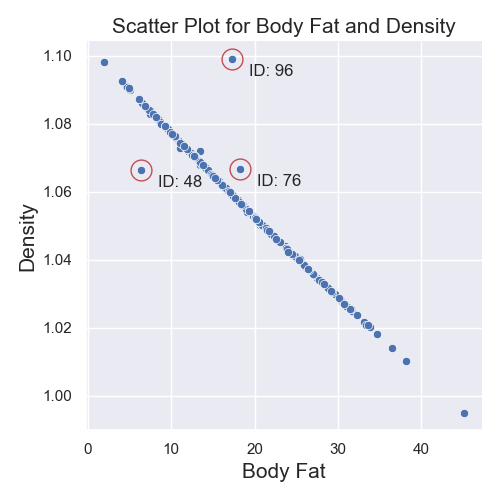
\includegraphics[width=0.425\textwidth]{../image/scatter_plot_for_density_and_fat.png}
   \hfill
   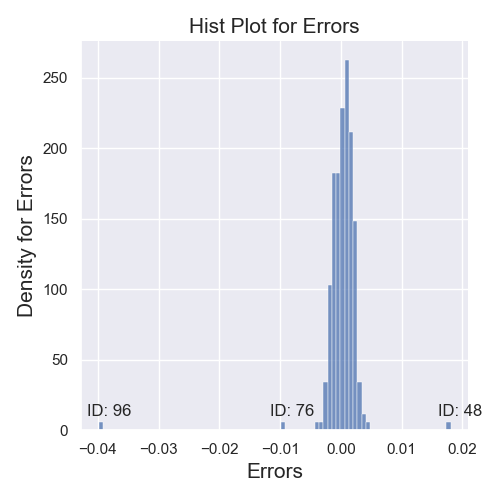
\includegraphics[width=0.425\textwidth]{../image/hist_plot_for_errors.png}
\end{figure}
\end{itemize}

\end{frame}


\begin{frame}{Summary of Data Cleaning}

\begin{itemize}
\item We use $3-\sigma$ criterion on the errors to find out these outliers. Finally, we use estimated body fat from Siri's equation to replace the original body fat for these samples.
\newline

\begin{tabular}{cccccc}
   \toprule
   IDNO & BODYFAT & Estimated Body Fat & Error\\
   \midrule
   48 & 6.4 & 14.1350 & 7.7350 \\
   76 & 18.3 & 14.0915 & -4.2085 \\   
   96 & 17.3 & 0.3685 & -16.9315 \\
   \bottomrule
\end{tabular}
\end{itemize}

\end{frame}

\begin{frame}{Feature Selection}

Here we consider two useful methods for the feature selection step: LASSO and stepwise regression.

\begin{itemize}
\item LASSO is use $L_1$ norm to keep the sparsity of the estimated solution. The features with non-zero coefficient are selected to be the important variables.

$$
L(\beta) = \Vert y-X\beta\Vert^2+\lambda \Vert\beta\Vert_1
$$

Finally, we select four features: Weight, Height, Abdomen and Thigh.

\end{itemize}
\end{frame}

\begin{frame}{Feature Selection}
\begin{itemize}

\item In general, the process of selecting variables by the stepwise regression method consists of two basic steps: one is to remove variables from the regression model that are not significant by t-test, and the other is to introduce new variables into the regression model that are significant by F-test.
\newline

Here, we set both thresholds for introducing and removing variables as $0.05$. Finally, we select four features: Weight, Wrist, Abdomen and Forearm.

\end{itemize}
\end{frame}

\begin{frame}{Model Selection}
\begin{itemize}
\item Candidate Models: Linear model with different predictors
\begin{align*}
\rm
Body Fat \sim Abdomen + Weight + Wrist + Forearm
\end{align*}
\centering
(Based on stepwise regression)
\begin{align*}
\rm
Body Fat \sim Weight + Height + Abdomen + Thigh
\end{align*}
\centering
(Based on Lasso method)
\end{itemize}

\begin{itemize}
\item Model performance result:
\end{itemize}

\centering
\begin{tabular}{cccccc}
   \toprule
   Model & Lasso Model & Stepwise Regression \\
   \midrule
   $R^2$ & 0.7245 & 0.7351 \\   
   MSE on test set (CV=6) & 18.228  & 17.208 \\
   \bottomrule
\end{tabular}
\end{frame}

\begin{frame}{Model Statistical Analysis}

\begin{center}
\begin{tabular}{cccc}
   \toprule
   Coefficients & Estimate & t value & p-value \\
   \midrule
   Intercept & -31.30 & -4.67 & $5.6\times 10^{-6}$ \\   
   Abdomen & 0.92  & 17.75 & $2.0\times 10^{-16}$\\
   Wrist & -1.39 & -3.40 & $8.0\times 10^{-4}$\\   
   Forearm & 0.45  & 2.65 & $8.5\times 10^{-3}$\\
   Weight & -0.13  & -5.48 & $1.05\times 10^{-7}$\\
   \bottomrule
\end{tabular}
\end{center}

\begin{center}
F-statistics = 162.4, p-value = $2.2\times 10^{-16}$
\end{center}

\begin{itemize}
\item T-test reports the significant partial effect of adding each predictors to the model.
\item F-test shows there exists relationship between response and predictors.
\end{itemize}
\end{frame}

\begin{frame}{Model Interpretation}
\begin{flushleft}
\textbf{Final Model}
\end{flushleft}
\begin{align*}
\rm
100\times Body fat \% = -31.30 + 0.92\times Abdomen -1.39\times Wrist \\
\rm
+0.45\times Forearm -0.13\times Weight
\end{align*}

\begin{flushleft}
\textbf{Some description of the final model in words:}
\end{flushleft}
 \begin{itemize}
    \item As men's abdomen increases by one centimeter, he is expected to gain 0.92\% in body fat.
    \item If two men have almost the same abdomen, forearm and weight, then having the smaller wrist means having the higher percentage of body fat.
\end{itemize} 

\end{frame}

\begin{frame}{Model Diagnostics}
\begin{flushleft}
\textbf{Assumptions for the SLR Model}
\end{flushleft}
\begin{itemize}
\item Linearity: The relationship between X and Y must be linear.
\item Independence of errors: There is not a relationship between the residuals and the Y variable;
\item Normality of errors: The residuals must be approximately normally distributed.
\item Homoskedasticity (Constant variance): The variance of the residuals is the same for all values of X.
\end{itemize}

\end{frame}

\begin{frame}{Model Diagnostics}
\begin{flushleft}
\textbf{Residual Plot}
\end{flushleft}
\begin{itemize}
\item We checked linearity, homoskedasticity and independence using Residual Plot. 

\begin{figure}
   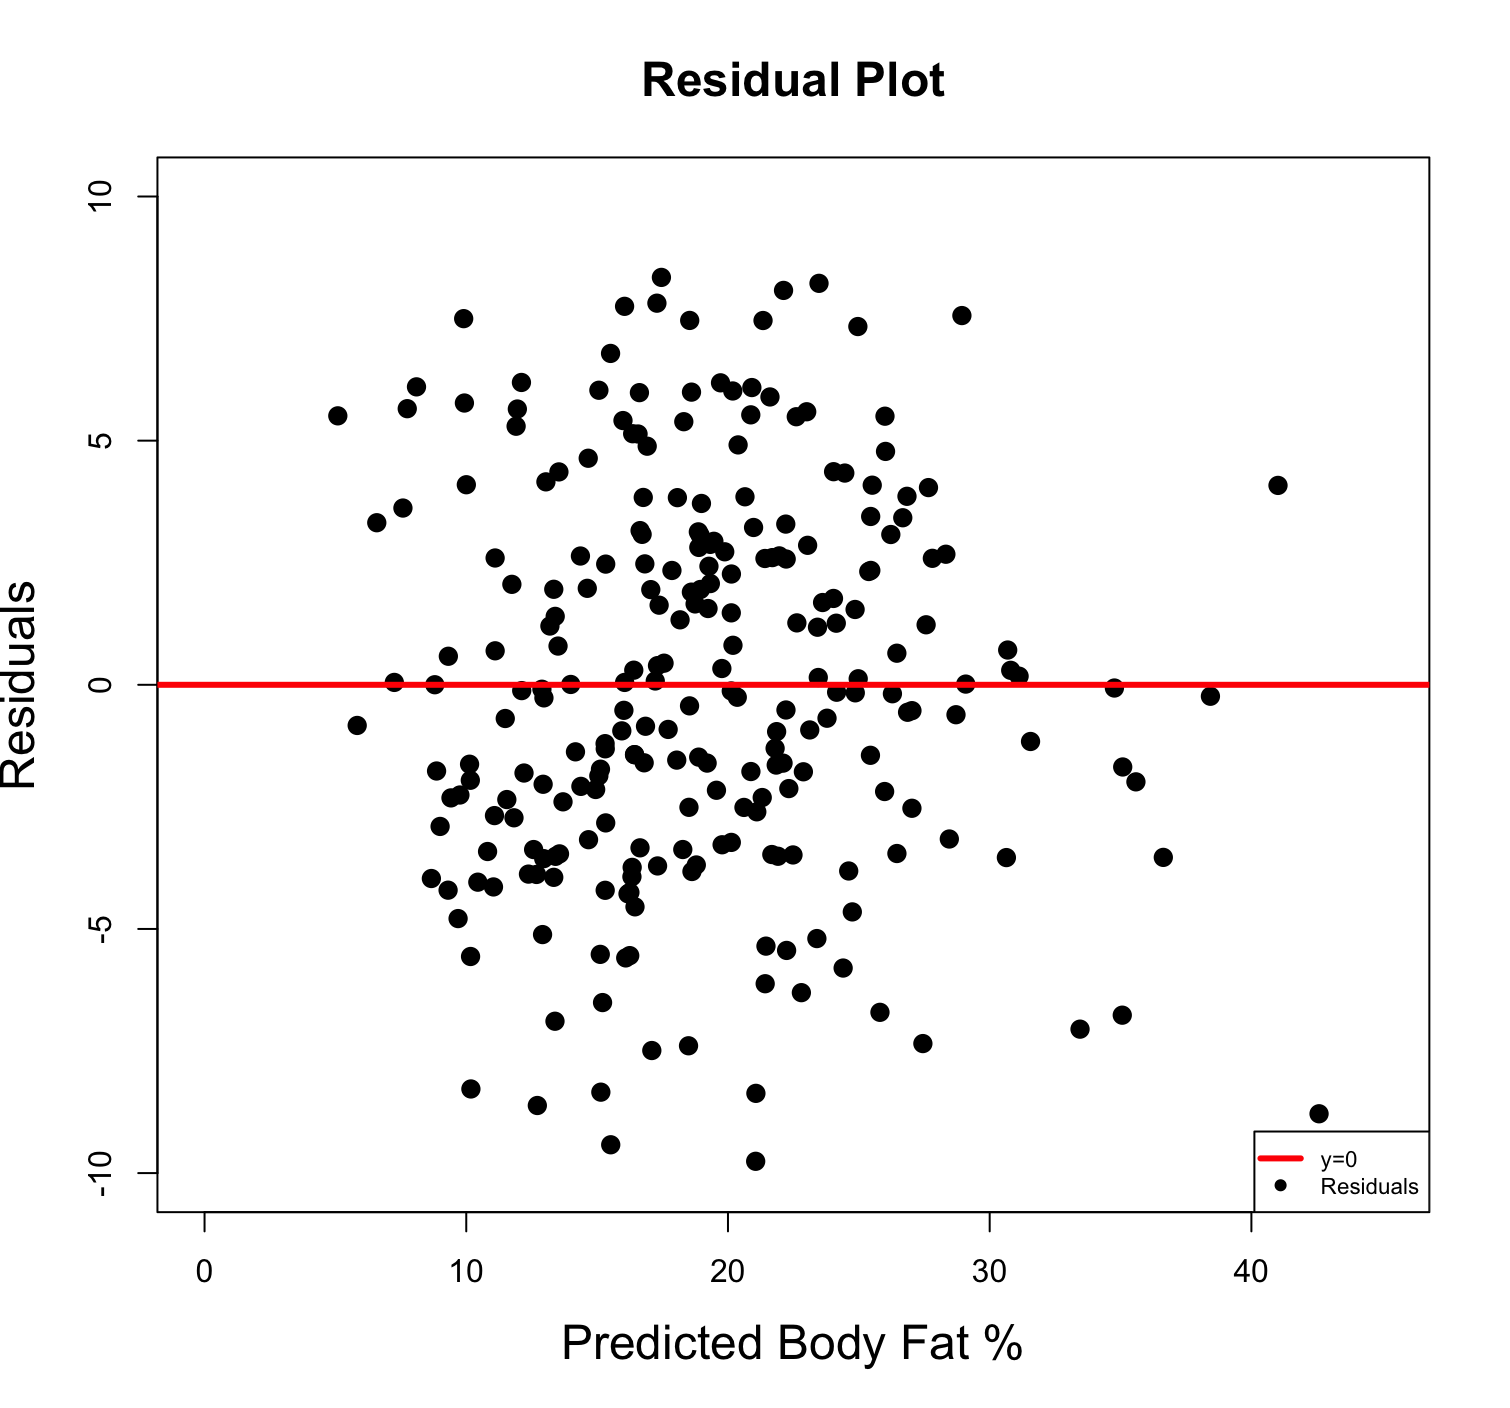
\includegraphics[width=0.425\textwidth]{../image/residual_plot.png}
\end{figure}
\end{itemize}


\end{frame}

\begin{frame}{Model Diagnostics}
\begin{flushleft}
\textbf{QQ Plot}
\end{flushleft}
\begin{itemize}
\item We checked normality using QQ Plot. 

\begin{figure}
   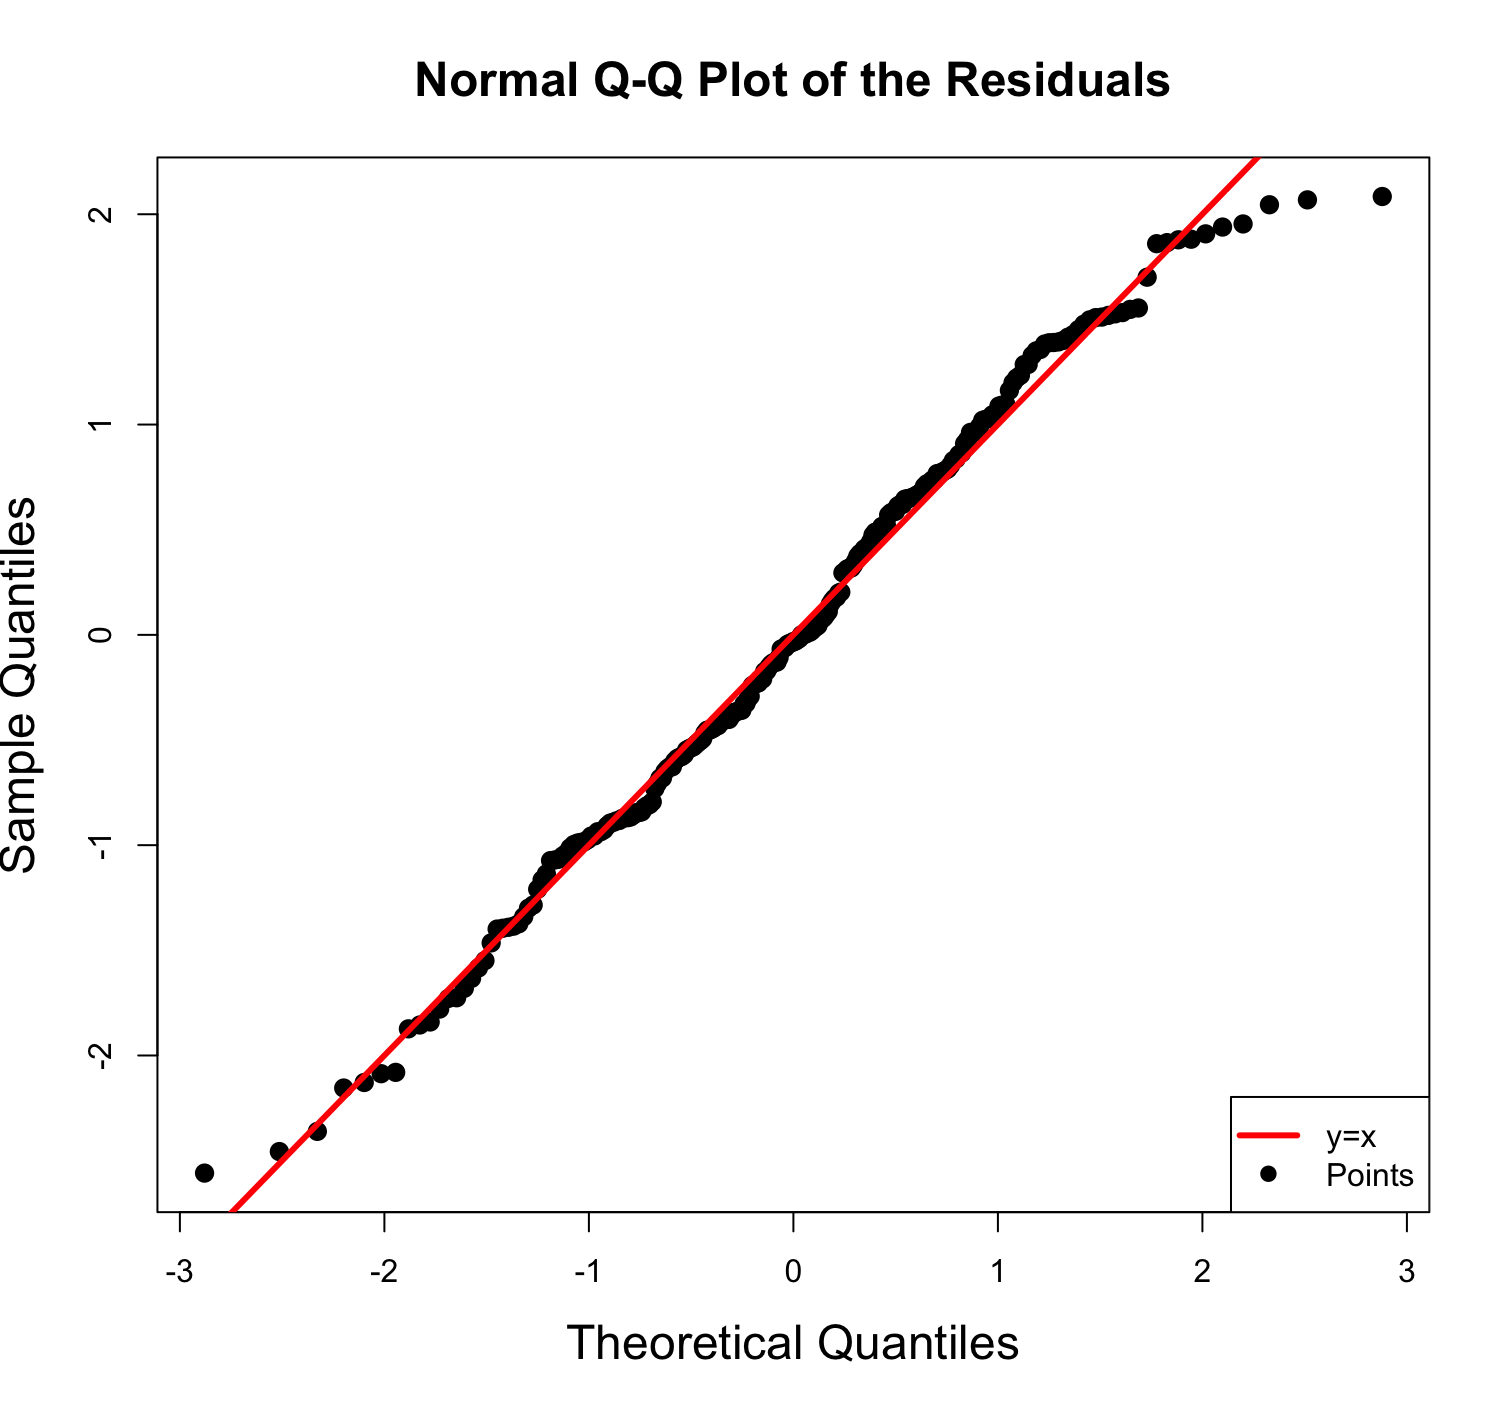
\includegraphics[width=0.425\textwidth]{../image/QQ_plot.png}
\end{figure}
\end{itemize}

\end{frame}

\begin{frame}{Model Diagnostics}
\begin{flushleft}
\textbf{Shapiro-Wilk test}
\end{flushleft}
\begin{itemize}
\item We used the Shapiro-Wilk test to test normality 

$$
\rm W=0.98926, p_{val}=0.05935
$$

\item We failed to reject "the sample is normal" because p-value is $0.05935>  0.05$. 
\end{itemize}

\end{frame}

\begin{frame}{Strength and Weekness}
\begin{itemize}
\item Strength
\begin{itemize}
\item Our model satisfies the linear regression assumption of homoskedasticity and linearity and it is explainable about its result.
\item The stepwise regression method overcomes the multiple linearity of predictors of the model.
\end{itemize}
\item Weekness
\begin{itemize}
\item The final model contains 4 predictors, which is kind of complicated.
\item If a man has extreme values, the model may produce negative body fat prediction.
\end{itemize}
\end{itemize}
\end{frame}

\end{document}
